\begin{minipage}[]{0.45\textwidth}

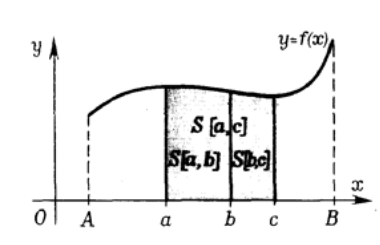
\includegraphics[scale=0.85]{pic4} \\
\textbf{Рисунок 4.} \\ \\ \\
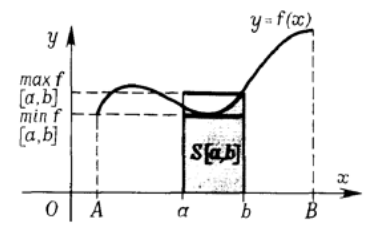
\includegraphics[scale=0.85]{images/pic5.png} \\
\textbf{Рисунок 5.} \\ \\ \\
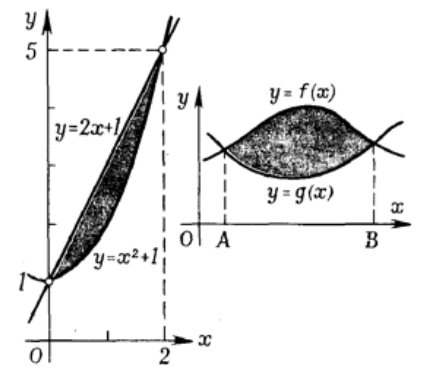
\includegraphics[scale=0.85]{images/pic67.png} \\
\textbf{Рисунок 6.} \ \ \ \ \ \ \ \ \ \ \ \ \ \ \ \ \ \ \ \textbf{Рисунок 7.}\\ \\ \\
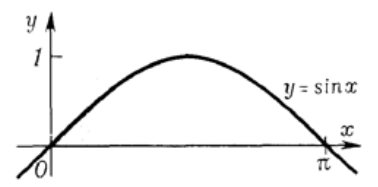
\includegraphics[scale=0.85]{images/pic8.png} \\
\textbf{Рисунок 8.} \\ \\ \\
\end{minipage}
\hfill
\hfill
\begin{minipage}[]{0.4\textwidth}
\parindent=0.6cm
\par
Непосредственно из определения интеграла следует, что функция про\-межутка $S$ -- интеграл от числовой функции $f$. В частности площадь всего подграфика функции $f$ равна \(\int_{A}^{B} f(x) \,dx\). Выведенная формула площади подграфика показывает геомет\-рический смысл интеграла: интеграл от неотрицательной функции -- это площадь подграфика этой функции. На этом основано использование ин\-теграла для вычисления площадей.
\indentВ качестве примера найдём площадь фигуры, отсекаемой от параболы $y = x^2+1$ прямой $y = 2x+1.$ \\
\indentПарабола и прямая пересекаются в точ\-ках, координаты которых (0, 1) и (2, 5) на\-ходятся как решения системы уравнений $y = x^2+1$, $y = 2x+1$. \\
\indentИскомая площадь (рис. 6) равна разности площадей подграфиков функций $x\rightarrow2x+1$ и $x\rightarrow x^2+1$, определённых на отрезке [0, 2]: \[S = \int_{0}^{2} (2x+1)\,dx \ - \int_{0}^{2} (x^2+1)\,dx =\] \\ \[= \int_{0}^{2} (2x+x^2)\,dx = 2\int_{0}^{2} x\,dx - \int_{0}^{2} x^2\,dx = \frac{4}{3}.\]
\indentВообще, если графики функций $f$ и $g$ пересекаются в точках с абциссами $A$ и $B$, а для всех чисел $x$ отрезка [$A, B$] выполнено неравенство $f(x) \geq g(x)$, то площадь фигуры, заключенной между этими подграфиками (рис. 7), равна $\int_{A}^{B} (f(x)-g(x))\,dx$. \\
\indent \textit{Упражнение 1. \ \ $a$) Вычислить площадь подграфика функций $x \rightarrow x^2$ на отрезке [0,1]. \\}
\indent \textit{$б$) Вычислить площадь, ограниченную аркой синусоиды и осью абцисс (рис. 8). \\}
\begin{center}
  \paragraph{2. Объем тела вращения}  
\end{center}
\parПредположим, что подграфик не\-отрицательный функции $f$, определен\-ной на отрезке [$A, B$], вращается вокруг оси абцисс. Каждому отрезку [$a, b$], содержащемуся в отрезке [$A,B$], поставим в соответствие число $V$ [$a, b$] -- объем части образовавше\-гося тела вращения, заключенной между плоскостями $x = a$ и $x = b$ (рис. 9).
\end{minipage}